\section{Siebensegmentanzeige}
\label{exercise7Segment}

Implementiere ein Programm, das die Zahlen 0 bis 99 auf der Siebensegmentanzeige ausgibt.
Nach jeder Ausgabe einer Zahl soll eine Pause eingelegt werden.

\begin{center}
	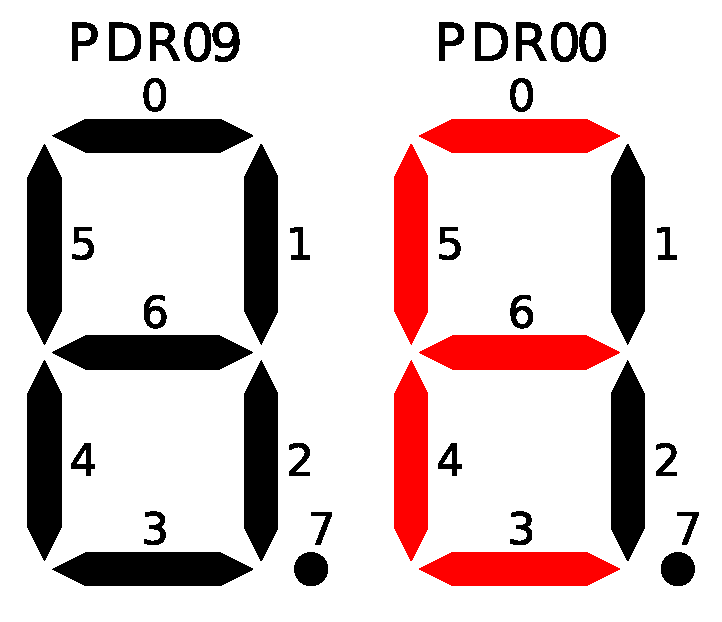
\includegraphics[width=0.2\textwidth]{figures/7seg_e}
\end{center}

Für die Ausgabe der Zahlen 0 bis 9 steht dir das Array \lstinline{DEC7SEG} zur Verfügung, welches die benötigten Werte für die jeweiligen Ziffern enthält.
Die beiden Anzeigen sind an den Ports 09 und 00 angeschlossen.
Die Ansteuerung erfolgt logisch invertiert, das bedeutet, dass ein Segment bei einer logischen 0 leuchtet und umgekehrt.
Beispiel: Ein \glqq{}E\grqq{} kann durch das Setzen der Pins 0, 3, 4, 5 und 6 (Binär: 10000110, bzw. Hexadezimal: 0x86) auf low gezeichnet werden. \\ \smallskip

Die Pause kann durch eine Schleife produziert werden, die in jedem Zyklus den Befehl \lstinline{__wait_nop()} aufruft.
Eine Konstante \lstinline{DELAY} steht dir für die Anzahl der Schleifendurchläufe zur Verfügung.
Achte insbesondere darauf, dass du für den Zähler den Datentyp \lstinline{long} verwendest.

\lstinputlisting{problems/listings/sevenseg.c}
